\hypertarget{a00005}{
\section{crf::crfNodeFactory Class Reference}
\label{a00005}\index{crf::crfNodeFactory@{crf::crfNodeFactory}}
}
This class generates the \hyperlink{a00043}{crf} Equalizer objects.  


{\tt \#include $<$crfNodeFactory.h$>$}

Inherits \hyperlink{a00013}{eqOsg::NodeFactory}.

Collaboration diagram for crf::crfNodeFactory:\nopagebreak
\begin{figure}[H]
\begin{center}
\leavevmode
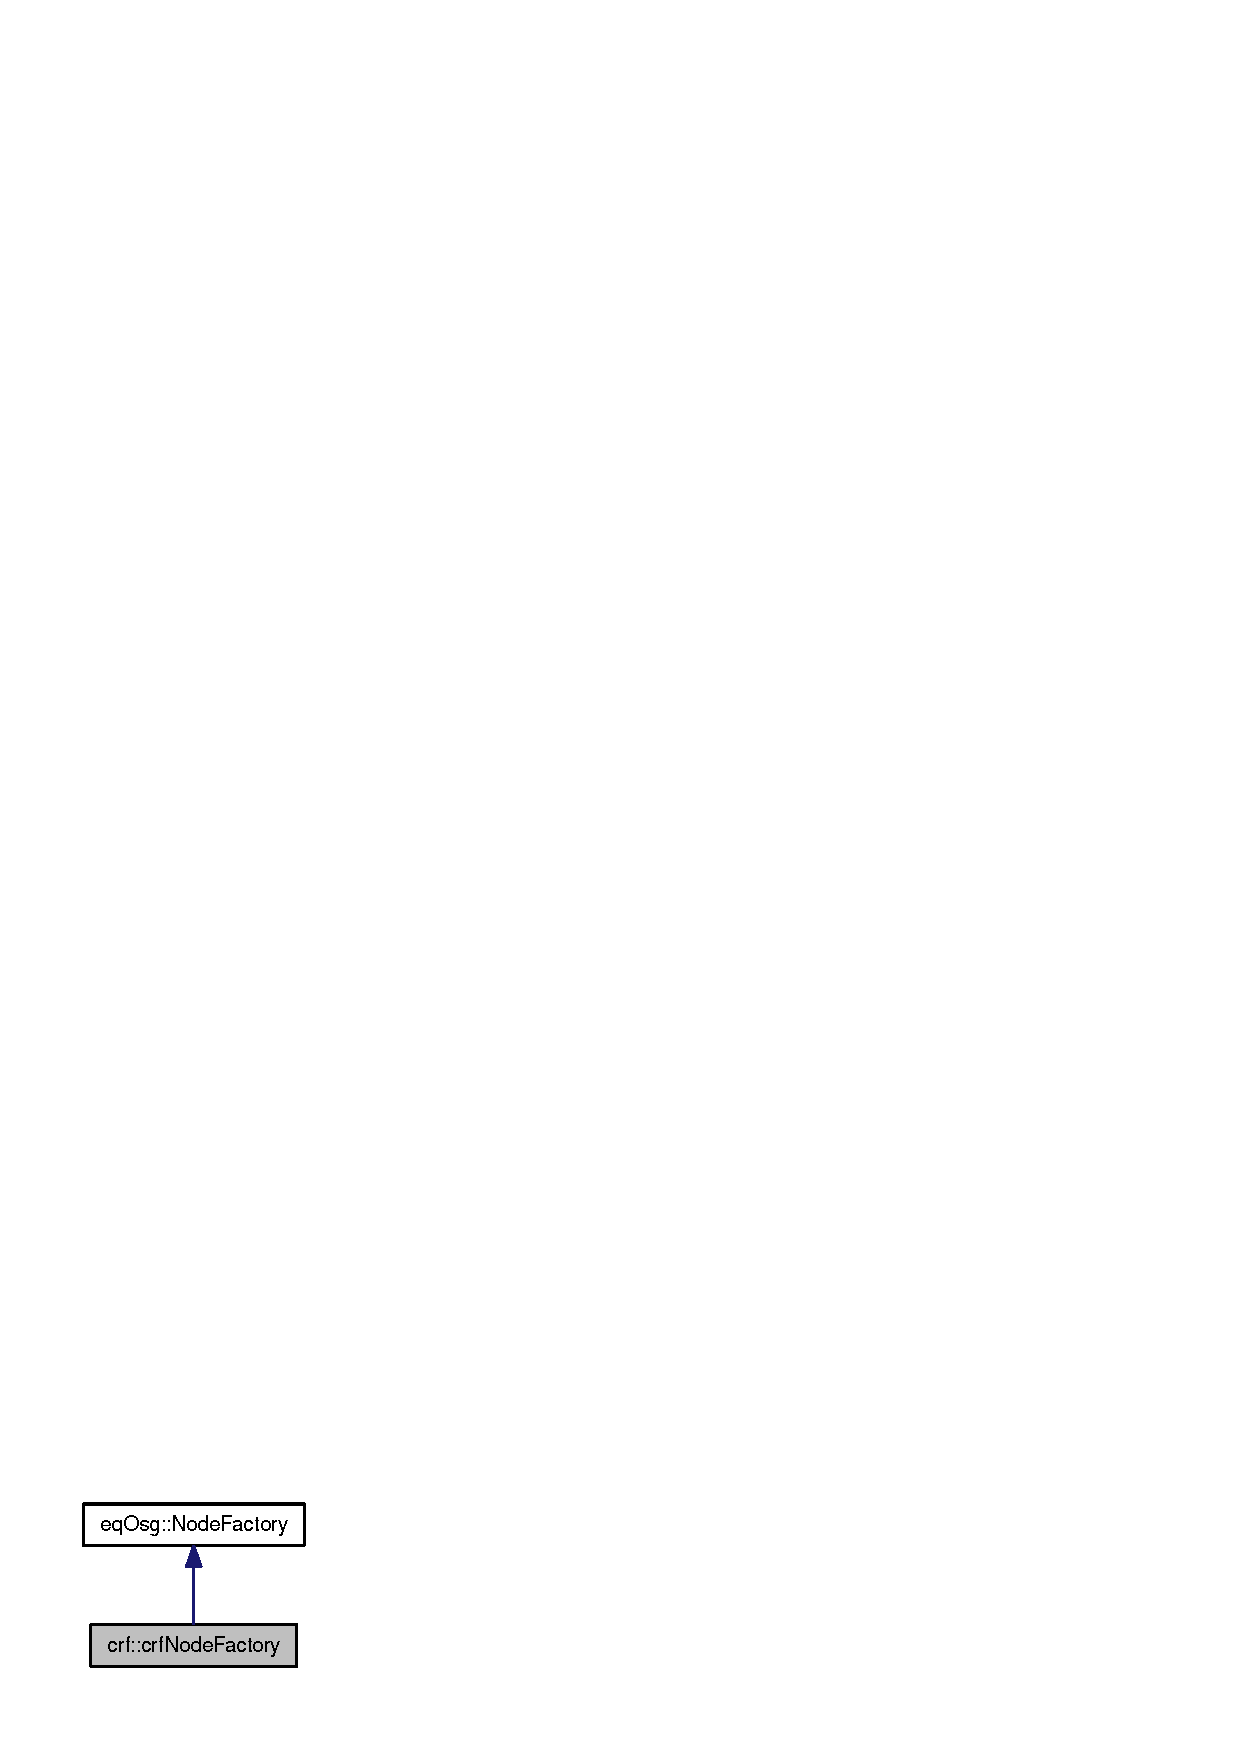
\includegraphics[width=150pt]{a00073}
\end{center}
\end{figure}
\subsection*{Public Member Functions}
\begin{CompactItemize}
\item 
\hypertarget{a00005_1361d01b702cda3adc2dc149fd4b9e58}{
\hyperlink{a00005_1361d01b702cda3adc2dc149fd4b9e58}{crfNodeFactory} ()}
\label{a00005_1361d01b702cda3adc2dc149fd4b9e58}

\begin{CompactList}\small\item\em Sets the sceneNode pointer to zero. \item\end{CompactList}\item 
virtual eq::Pipe $\ast$ \hyperlink{a00005_5f35c307f323b385869226c6083df93d}{createPipe} (eq::Node $\ast$parent)
\begin{CompactList}\small\item\em Creates the \hyperlink{a00006}{crfPipe} objects. \item\end{CompactList}\item 
virtual eq::Config $\ast$ \hyperlink{a00005_0b7b562ae3d0ccc5a98017195926057f}{createConfig} (eq::ServerPtr parent)
\begin{CompactList}\small\item\em Initialises the \hyperlink{a00004}{crfConfig}. \item\end{CompactList}\item 
void \hyperlink{a00005_52740ca913279f9cbdfc4a10f55b691d}{setSceneNode} (osg::ref\_\-ptr$<$ osg::Node $>$ node)
\begin{CompactList}\small\item\em Sets the pipes root node. \item\end{CompactList}\end{CompactItemize}


\subsection{Detailed Description}
This class generates the \hyperlink{a00043}{crf} Equalizer objects. 

\begin{Desc}
\item[See also:]\hyperlink{a00013}{eqOsg::NodeFactory} \end{Desc}


\subsection{Member Function Documentation}
\hypertarget{a00005_0b7b562ae3d0ccc5a98017195926057f}{
\index{crf::crfNodeFactory@{crf::crfNodeFactory}!createConfig@{createConfig}}
\index{createConfig@{createConfig}!crf::crfNodeFactory@{crf::crfNodeFactory}}
\subsubsection[{createConfig}]{\setlength{\rightskip}{0pt plus 5cm}virtual eq::Config$\ast$ crf::crfNodeFactory::createConfig (eq::ServerPtr {\em parent})\hspace{0.3cm}{\tt  \mbox{[}inline, virtual\mbox{]}}}}
\label{a00005_0b7b562ae3d0ccc5a98017195926057f}


Initialises the \hyperlink{a00004}{crfConfig}. 

\begin{Desc}
\item[See also:]eqOsg::Nodefactory::createConfig \end{Desc}


Reimplemented from \hyperlink{a00013_0e80614084de6b23a4a2677fc8af7f93}{eqOsg::NodeFactory}.\hypertarget{a00005_5f35c307f323b385869226c6083df93d}{
\index{crf::crfNodeFactory@{crf::crfNodeFactory}!createPipe@{createPipe}}
\index{createPipe@{createPipe}!crf::crfNodeFactory@{crf::crfNodeFactory}}
\subsubsection[{createPipe}]{\setlength{\rightskip}{0pt plus 5cm}virtual eq::Pipe$\ast$ crf::crfNodeFactory::createPipe (eq::Node $\ast$ {\em parent})\hspace{0.3cm}{\tt  \mbox{[}inline, virtual\mbox{]}}}}
\label{a00005_5f35c307f323b385869226c6083df93d}


Creates the \hyperlink{a00006}{crfPipe} objects. 

If a osg::Node is set, the node will be passed to the new pipe. \begin{Desc}
\item[See also:]\hyperlink{a00013_10e06f5d0d32f146994274682d39e666}{eqOsg::NodeFactory::createPipe} \end{Desc}


Reimplemented from \hyperlink{a00013_10e06f5d0d32f146994274682d39e666}{eqOsg::NodeFactory}.\hypertarget{a00005_52740ca913279f9cbdfc4a10f55b691d}{
\index{crf::crfNodeFactory@{crf::crfNodeFactory}!setSceneNode@{setSceneNode}}
\index{setSceneNode@{setSceneNode}!crf::crfNodeFactory@{crf::crfNodeFactory}}
\subsubsection[{setSceneNode}]{\setlength{\rightskip}{0pt plus 5cm}void crf::crfNodeFactory::setSceneNode (osg::ref\_\-ptr$<$ osg::Node $>$ {\em node})\hspace{0.3cm}{\tt  \mbox{[}inline\mbox{]}}}}
\label{a00005_52740ca913279f9cbdfc4a10f55b691d}


Sets the pipes root node. 

If this node is set, this node will be passed to the pipe. \begin{Desc}
\item[Parameters:]
\begin{description}
\item[{\em node}]The to set osg scene node \end{description}
\end{Desc}


The documentation for this class was generated from the following file:\begin{CompactItemize}
\item 
E:/schule/Thesis/Repo/trunk/crf/src/crfNodeFactory.h\end{CompactItemize}
